
\vspace{\baselineskip}
\section{penjelasan tentang catatan kaki dan fungsinya}

\vspace{\baselineskip}
Yang dimaksud dengan catatan kaki adalah daftar keterangan khusus yang ditulis pada bagian paling bawah disetiap lembaran akhir bab karya ilmiah (makalah, skripsi, tesis dll). Atau catatan kaki merupakan keterangan refrensi yang ditempatkan pada kaki tulisan atau teks karya ilmiah.\par

\vspace{\baselineskip}
Berikut ini beberapa fungsi dari catatan kaki yang diantaranya seperti:\par


\vspace{\baselineskip}
\noindent Catatan kaki berfungsi untuk memberikan keterangan dan penjelasan tentang sumber dari kutipan penyusunan daftar bacaan pada karya ilmiah supaya dapat dimengerti oleh pembaca.\par

\vspace{\baselineskip}
\noindent untuk menghargai sumber kutipan yang dikutip, supaya pembaca karya ilmiah mengetahui sumber kutipan yang digunakan\par

\vspace{\baselineskip}
\noindent Dan untuk menunjukan refrensi lain supaya pembaca karya ilmiah dapat mengetahui ulasan yang lebih jelas mengenai istilah yang digunakan\par

\vspace{\baselineskip}
\subsection{cara penulisan catatan kaki}

\vspace{\baselineskip}
\noindent Bagaimana cara menulis catatan kaki?\par

\vspace{\baselineskip}
Dalam penulisannya, catatan kaki memiliki aturan-aturan yang perlu diperhatikan. Hal-hal tersebut diterapkan supaya dapat dimengerti oleh para pembaca karya ilmiah. Dalam menulis catatan kaki ada beberapa hal yang perlu diperhatikan, yang diantaranya:\par

\begin{itemize}
	\vspace{\baselineskip}
	\item Penulisannya dipisahkan oleh garis yang panjangnya 14 karakter dari margin sebelah kiri dan berjarak 4 spasi dari tulisan atau teks.\par

\vspace{\baselineskip}
	\item Diketik atau ditulis dengan satu spasi.\par

\vspace{\baselineskip}
	\item Harus diberikan nomer.\par

\vspace{\baselineskip}
	\item Nomer pada catatan kaki diketik dengan jarak 6 karakter dari margin sebelah kiri.\par

\vspace{\baselineskip}
	\item Kalau catatan kakinya lebih dari satu baris, maka pada baris yang kedua maupun selanjutnya dimulai seperti margin teks yang biasanya tepat pada margin bagian sebelah kiri.\par

\vspace{\baselineskip}
	\item Kalau catatan kakinya lebih dari satu maka jarak antar catatan kaki dengan catatan kaki yang lainnya sama seperti jarak spasi pada teks.\par

\vspace{\baselineskip}
	\item Catatan kaki harus ditulis pada halaman yang sama, jika terlalu panjang lebih baik potong teksnya daripada memotong catatan kaki.\par

\vspace{\baselineskip}
	\item Berjarak 3 centimeter dengan margin bagian bawah, seperti halnya pada aturan teks.\par

\vspace{\baselineskip}
	\item Jika nama pengarang dua sampai tiga orang, maka harus ditulis semuanya. Sedangkan jika nama pengarangnya lebih dari tiga orang maka tulis saja nama pengarang yang pertama lalu dibelakangnya ditulis et.al., atau dkk.\par

\vspace{\baselineskip}
	\item Nama pengarang harus ditulis sesuai nama aslinya, pangkat dan gelar tidak perlu ditulis.\par

\vspace{\baselineskip}
	\item Judul buku atau sumber harus diberi garis bawah, jika diketik dengan komputer maka harus dicetak miring.\par

\vspace{\baselineskip}
Footnotes Merupakan catatan kaki dalam penulisan pada latex \par

\vspace{\baselineskip}
Berikut adalah contoh code latex:\par

\vspace{\baselineskip}
Coding pembuatan catatan kaki\par

\vspace{\baselineskip}
$documentclass$ \{ $article$ \} \par

$begin$ \{ $document$ \} \par

$title$ \{ $google$ \} \par

\vspace{\baselineskip}
Penjelasan syntax yang tadi di pakai adalah sebagai berikut :\par

\vspace{\baselineskip}
$Documenclass$ \{ $article$ \} \par

\vspace{\baselineskip}
	\item Untuk menentukan jenis halaman (kita menggunakan article)\par

$begin$ \{ $document$ \} \par

\vspace{\baselineskip}
	\item Untuk memulai document\par

$title$ \{ $google$ \} \par

\vspace{\baselineskip}
	\item Untuk membuat judul teks, yaitu ‘google’\par

$maketitle$\par

\vspace{\baselineskip}
-Untuk menampilkan judul\par

\vspace{\baselineskip}
$footnote$ \{ $teks$ \} \par

\vspace{\baselineskip}
	\item Untuk membuat catatan kaki tersebut\par

\vspace{\baselineskip}
$end$ \{ $document$ \} \par
	\item Untuk mengakhiri document\par

\vspace{\baselineskip}
Coding yang akan digunakan sebagai berikut :\par

\vspace{\baselineskip}
Documentclass \{ $article$ \} \par

\vspace{\baselineskip}
Begin \{ $document$ \} \par

\vspace{\baselineskip}
$end$ \{ $document$ \} \par

\vspace{\baselineskip}
Penjelasan syntax yang tadi di gunakan berikut penjelasan nya:\par

\vspace{\baselineskip}
$documenclass$ \{ $article$ \} \par

\vspace{\baselineskip}
	\item Untuk menentukan jenis halaman\par


$begin$ \{ $document$ \} \par

	\item Untuk memulai dokumen\par

\vspace{\baselineskip}
$flushleft$\par

	\item Untuk penulisan rata kiri\par

\vspace{\baselineskip}
$\$$\par

	\item Untuk syarat penulisan rumus (di awal dan di akhir)\par

\vspace{\baselineskip}
$ \string^ $\par

	\item Untuk penulisan pangkat atau superscript\par

\vspace{\baselineskip}
$ \_ $\par

	\item Untuk penulisan index atau subscript\par

\vspace{\baselineskip}
$frac$\par

	\item Untuk menuliskan pecahan\par

\vspace{\baselineskip}
$pm$\par

-Untuk penulisan plus minus\par

\vspace{\baselineskip}
$sqrt$\par

	\item Untuk penulisan akar\par

\vspace{\baselineskip}
$alpha$\par

\vspace{\baselineskip}
	\item Untuk menuliskan symbol alpa
	
\end{itemize}\par

\vspace{\baselineskip}
Jadi xxx itu adalah penulisan kata-kata sendiri jadi isi sendiri agar tidak ditiru atau di modif sembarangan\par

\vspace{\baselineskip}
\noindent Penjelasan tentang footnote atau pembuatan catatan kaki\par

\vspace{\baselineskip}
Verbatim berfungsi untuk membuat kalimat atau karakter yang di tulis\par

\vspace{\baselineskip}
Table berfungsi membuat table\par

\vspace{\baselineskip}
4.6.1 pembuatan list dan item pembuatan daftar berurutan untuk membuat daftar yang berurutan\par

\vspace{\baselineskip}
Jadi penulisan yang tepat yaitu menggunakan\par

\vspace{\baselineskip}
Documentclass[12pt,a4paper,oneside,bahasa,dvips] book atau begin document halo, jadi penjelasan nya kita akan membuat dokumen dengan ukuran kertas a4, selanjutnya buku tersebut akan ditampilkan kedalam bahasa Indonesia, dan daftar tersebut akan di susun secara otomatis pada awal dokumen\par


\vspace{\baselineskip}
\noindent 1.4 Hal penting untuk mengatur dokumen atau margin\par

\vspace{\baselineskip}
keterangan yang akan di terangkan berupa\par


\vspace{\baselineskip}
\noindent documentclass\par


\begin{itemize}

\vspace{\baselineskip}
	\item tadi yang menentukan dokumen apa yang akan anda buat\par

\vspace{\baselineskip}
12pt\par

	\item Ukuran huruf\par

\vspace{\baselineskip}
A4paper\par

	\item Jenis\par

\vspace{\baselineskip}
Titlepage\par

	\item Judul terpisah dengan isi\par

\vspace{\baselineskip}
Notitlepage\par

	\item Judul tidak terpisah dengan isi\par

\vspace{\baselineskip}
Oneside\par

	\item Satu sisi\par

\vspace{\baselineskip}
Twocolomn\par

	\item Tampilan dokumen\par

\vspace{\baselineskip}
Bahasa\par

	\item Bahasa Indonesia
	\vspace{\baselineskip}
	
\end{itemize}\par

\vspace{\baselineskip}
\noindent 1.5 Setelah melakuka itu kita bisa membuat sebuah title\par

\vspace{\baselineskip}
\noindent $title$ \{ a \} \par

\vspace{\baselineskip}
\noindent maketitle\par

\begin{itemize}
	
	\vspace{\baselineskip}
	\item Jadi yang di dalam kurung itu isi sesuia yang di inginkan kalian\par

\vspace{\baselineskip}
1.6 Membuat author\par

\vspace{\baselineskip}
	\item Letakan kode nya diantara title dan maketitle lalu isi dalam kurung tersebut nama pengarang\par

\vspace{\baselineskip}
$author$ \{ a \} \par

	\item Jadi sebenernya author juga berfungsi dengan enter\par

\vspace{\baselineskip}
1.7 Cara membuat judul\par
\begin{verbatim}
	
part l

section l  

subsection  l 
\end{verbatim}

\vspace{\baselineskip}
	\item Dalam kurung isi dengan judul yang di buat\par

\vspace{\baselineskip}
1.8 Penomoran dokumen\par
\begin{verbatim}

begin \{ enumerate \}

item

item

item

$end$ \{ enumerate \}
\end{verbatim}

\vspace{\baselineskip}
1.9 Bila ingin menambahkan footnote bisa ditambahkan code nya\par

\vspace{\baselineskip}
footnote \{ l \} \par

\vspace{\baselineskip}
	\item Contoh lain dari footnote adalah\par

$footnote$ \{ $…$ \} \par

\vspace{\baselineskip}
	\item Kurung tersebut bisa di isi dan di sesuaikan dengan keinginan masing masing\par

$documentclass$ \{ $article$ \} \par

$begin$ \{ $document$ \} \par

Bla bla bla.$footnote$ \{ $ini footnote.$ \} \par

$end$ \{ $document$ \} \par

\vspace{\baselineskip}
Maka hasil nya akan bla bla bla ada pangkatnya di atas kata kata blabla bla tersebut\par

\vspace{\baselineskip}
Ini adalah penulisan dan penjelasan catatn kaki tujuan nya agar pembaca mengetahui fungsi dari catatan kaki dalam pembuatan karya ilmiah\par
\begin{itemize}
	\item isal1
\end{itemize}
\begin{figure}[ht]
	\centerline{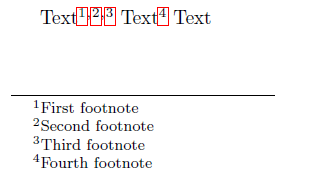
\includegraphics[width=0.70\textwidth]{gambar/isal1}}
	\caption{penulisan catatan kaki}
	\label{catatan kaki}
\end{figure}
\subsection{kesalahan dalam penulisan catatan kaki menurut kaidah EYD}
\begin{itemize}
	
	\vspace{\baselineskip}
	\item Eveline Siregar dan Hartini Nara, Teori Belajar Dan Pembelajaran, (Bogor:Ghalia Indonesia, 2010)hal 4
\end{itemize} 

\vspace{\baselineskip}
Perbaikan nya seperti ini\par

\vspace{\baselineskip}
Eveline Siregar dan Hartini Nara, Teori Belajar Dan Pembelajaran (bogor: Ghalia Indonesia. 2010),hlm.4.\par

\vspace{\baselineskip}
Kesalahan:\par
\begin{itemize}
	\vspace{\baselineskip}
	\item Taniredja, Tukiran, Efi, dan Sri, Metode-metode pembelajaran inovatif (Bandung:Alfabeta.2011)hal 23
\end{itemize}

\vspace{\baselineskip}
Perbaikan nya seperti ini\par

\vspace{\baselineskip}
TAniredja, Tukiran ,Efi, dan Sri, Metode-metode pembelajaran inovatif\par

(Bandung:Alfabeta,2011), hlm 23.\par

\vspace{\baselineskip}
Jadi pengertian catatan kaki adalah keterangan-keterangan atas teks/naskah/tulisna yang ditempatkan pada kaki halaman tulisan yang bersangkutan\par

(keraf, 2004:218)\par

\vspace{\baselineskip}
2.2 Tujuan nya adalah\par

\vspace{\baselineskip}
Catatan kaki tidak hanya sebagai bukti bahwa tulisan kita berasal dari buku lain melainkan ada banyak tujuannya antara lain:\par

\vspace{\baselineskip}
	\item Pembuktian menunjukan tempat/sumber bahwa yang disebutkan pada tulisan telah dibuktikan orang lain.\par

\vspace{\baselineskip}
	\item Memberi apresiasi penghargaan, rasa terima kasih pada orang yang telah dikutipnya\par

\vspace{\baselineskip}
	\item Menyampaikan keterangan tambahan memperkuat uraian di luar persoaalan dalam teks, biasanya berupa: inti cerita, informasi tambahan
\end{itemize}\par

\vspace{\baselineskip}
\noindent Merujuk bagian lain dalam tulisan dalam tulisan referensi melihat bagian lain dalam tulisannya, biasanya dengan singkatan-singkatan tertentu\par

\vspace{\baselineskip}
\noindent Contoh lain yang bisa kita lihat adalah\par

\vspace{\baselineskip}
\noindent Cara penulisan atau pencantuman nama\par


\begin{itemize}
\vspace{\baselineskip}
	\item pengarang (tanpa dibalik)\par

\vspace{\baselineskip}
Judul(dicetak miring atau jika ditulis tangan digaris bawah)\par

\vspace{\baselineskip}
Data publikasi (meliputi kota terbit kemudian titik dua (:) kemudian penerbit koma (,) tahun terbit\par

\vspace{\baselineskip}
Nomor halaman\par

\vspace{\baselineskip}
2.3 Atau bisa disebut juga keterangan atas teks karangan yang di tempatkan pada kaki halaman karangan yang bersangkutan (Gorys Keraf, 1994:193). Catatan kaki dapat berupa rujukan bahan penulisan yang dijadikan sumber dan dapat pula berupa keterangan tambahan.\par

\vspace{\baselineskip}
Fungsinya berupa\par

\vspace{\baselineskip}
	\item Catatan kaki yang berupa referensi\par

\vspace{\baselineskip}
	\item Fungsi akademis\par

\vspace{\baselineskip}
	\item Memberikan dukungan argumentasi atau pembuktian\par

\vspace{\baselineskip}
	\item Pembuktian(rujukan) kutipan naskah\par

\vspace{\baselineskip}
	\item Memperluas makna informasi bahasan dalam naskah\par

\vspace{\baselineskip}
	\item Kebenerana fakta\par

\vspace{\baselineskip}
	\item Kualitas karangan\par

\vspace{\baselineskip}
	\item Penilaian sumber data\par

\vspace{\baselineskip}
	\item Pembedaan data pusaka dan keterangan tambahan\par

\vspace{\baselineskip}
	\item Mencegah pengulangan data pustaka\par

\vspace{\baselineskip}
	\item Memudahkan peninjauan penggunaan referensi\par

\vspace{\baselineskip}
	\item Penyunting data pustaka\par

\vspace{\baselineskip}
	\item Menunjukan kualitas kecerdasan akademis penulisan\par

\vspace{\baselineskip}
	\item Etika atau moral\par

\vspace{\baselineskip}
	\item Pengakuan dan penghargaan kepada penulis\par

\vspace{\baselineskip}
	\item Kualitas ilmiah\par

\vspace{\baselineskip}
	\item Kecermatan lebih akurat\par

\vspace{\baselineskip}
	\item Intelektual bukan plagiat\par

\vspace{\baselineskip}
	\item Kesantunan akademis penulisan\par

\vspace{\baselineskip}
	\item Tempat catatan kaki\par

\vspace{\baselineskip}
	\item Uraian pada halaman yang sama pada bagian bawah digunakan dalam skripsi dan lain lain\par

\vspace{\baselineskip}
	\item Uraian catatan bab terakhir untuk karangan popular\par

\vspace{\baselineskip}
	\item Penempatan catatan kaki harus konsisten. Misalnya, penempatan catatan kaki pada kaki halaman pertama. Penempatan ini dilakukan seterusnya dengan cara yang sama sampai dengan halaman terakhir.
\end{itemize}\par

\vspace{\baselineskip}
\noindent 2.4  Penulisan catatan kaki\par

\begin{itemize}
	\vspace{\baselineskip}
	\item Dipisah tiga sepasi dari naskah yang sama\par

\vspace{\baselineskip}
	\item Antaracatatan kaki dipisahkan dengan satu spasi\par

\vspace{\baselineskip}
	\item Diketik sejajar dengan margin
\end{itemize}\par

\vspace{\baselineskip}
\noindent Itu adalah cara tips untuk mengetahui catatan kaki dan bagaimana penerapan pada latex tersebut maka ikuti langkah diatas maka akan kalian ketahui hasilnya selain itu pembelajaran diatas didapatkan di halaman internet untuk pemahaman lebih jelasnya bisa buka halaman cara penulisan bahasaindonesia di browser pembaca terimakasih\par
